% -*- TeX -*- -*- US -*-
\documentclass[12pt]{article}
\input{sl_preamble.tex}
\input{sl_graphics_preamble.tex}
\graphicspath{{Figures/}}
\usepackage{mciteplus}
\usepackage{titling}
\setlength{\droptitle}{-1.5in}
\renewcommand{\maketitlehookd}{\vspace*{-0.5in}}
%\usepackage{abstract}
%\renewcommand{\abstractname}{Summary}
%\renewcommand{\abstractnamefont}{\normalfont\large\bfseries}
%\renewcommand{\abstracttextfont}{\normalfont}
%\renewcommand{\absnamepos}{flushleft}
%\setlength{\absleftindent}{0in}
%\setlength{\absrightindent}{0in}
% ----------------------------------------------------------------
% New commands etc.
\input{sl_definitions.tex}
%\input{sl_symbols.tex}



%%%%%%%%%%%%%%%%%%%%%%%%%%%%%%%%%%%%%%%%%%%%%%%%%%%%%%%%%%%%%%%%%%%%%%%%%%
% Title info:
\title{Learning and memory with complex synapses}
%
% Author List:
%
\author{Subhaneil Lahiri and Surya Ganguli}
%\author{Subhaneil Lahiri\thanks{\emaillink{sulahiri@stanford.edu}}~ and Surya Ganguli\thanks{\emaillink{sganguli@stanford.edu}}\\
%%
%\small{
%Department of Applied Physics, Stanford University, Stanford CA
%}
%}
\date{}

\begin{document}

\maketitle


%%%%%%%%%%%%%%%%%%%%%%%%%%%%%%%%%%%%%%%%%%%%%%%%%%%%%%%%%%%%%%%%%%%%%%%%%%

%\begin{abstract}
\subsection*{Summary}

We consider the storage of long term memories through synaptic modifications in existing networks.
Recent experimental work suggests that single synapses are digital, in the sense that, from the perspective of extracellular physiology, they can only take on a finite number of discrete values for their strength.
This imposes catastrophic limits on the memory capacity of classical models of memory that have relied on a continuum of analog synaptic strengths [Amit and Fusi, Network: Computation in Neural Systems (1992)]\nocite{amit1992constraints}.

However, synapses have many internal molecular states [Coba et al., Sci Signal (2009)]\nocite{Coba2009phosphorylation}, suggesting we should model synapses themselves as complex molecular networks, rather than by a single scalar value, or strength.
We develop new theorems bounding the memory capacity of such complex synaptic models and describe the structural organization of internal molecular networks necessary for achieving these limits.

In particular, we prove an upper bound on the area under the signal-to-noise ratio (SNR) curves for \emph{all} models of this type, as well as the SNR at any fixed time and the memory capacity of these synapses.

This type of exploration of the space of possible synaptic models should prove to be essential for understanding the internal molecular structure of real synapses.
%\end{abstract}

\subsection*{Additional detail}

Much of the previous work on complex synapses has focused on the study of specific models \cite{amit1994learning,*Fusi2005cascade,*Fusi2007multistate}.
If we wish to understand the structure of the molecular networks responsible for synaptic plasticity, it will be vital to have explored the space of all possible molecular networks so that we can develop a correspondence between features of these networks and desirable/undersirable properties of the synapse.

\begin{figure}
 \begin{center}
 \begin{myenuma}
   \item\aligntop{\includegraphics[width=4cm]{synapse.svg}}\label{fig:synapse}
   \hspace{0.25cm}
   \item\aligntop{\includegraphics[width=2cm]{pot.svg}}\label{fig:pot}
   \hspace{0.25cm}
   \item\aligntop{\includegraphics[width=2cm]{dep.svg}}\label{fig:dep}
 \end{myenuma}
 \end{center}
 \caption{Models of complex synapses. (\ref{fig:synapse}) The complex synapse has a number of internal states, some of which correspond to a strong synaptic strength and some to weak. (\ref{fig:pot},\ref{fig:dep}) Potentiation and depression induce stochastic transitions between these states.}\label{fig:compsynapse}
\end{figure}

We model synaptic plasticity with two Markov processes between the internal states, one for potentiation and one for depression (see \fref{fig:compsynapse}).
These are responsible for the initial creation of a memory and the subsequent forgetting due to ongoing plasticity.
The performance of the synapse is quantified by the signal-to-noise ratio (SNR) as a function of time.

We can use the transition probabilities to optimize features of the SNR, thereby proving upper limits on the performance of the synapse.
For example we show that the area under the curve has an upper bound that grow linearly with the number of internal states.
This upper limit is saturated by a particular transition network with a linear chain topology,
We also find an upper limit on the instantaneous value of the SNR at any time.
This allows us to bound the length of time that any memory can be recovered, and hence the memory capacity of such synapses.

The models that maximize the SNR at one time are shown to be dominated by a single time-scale.
When this is extended to maximizing the SNR at several, well separated times, we are led to models with multiple time-scales.

%%%%%%%%%%%%%%%%%%%%%%%%%%%%%%%%%%%%%%%%%%%%%%%%%%%%%%%%%%%%%%%%%%%%%%%%%%

\bibliographystyle{utcaps_m}
\bibliography{Abstract-minimal}
%\bibliography{maths,neuro}

\end{document}
